\section{Benchmarks}
\label{sec:benchmark}

Our framework includes 3 main parts: algorithms for path searching, schedule to order messges into a sending queue an, transport to transfer message between nodes. We first show our performance studies each part from the bottom of the framework to the top. We then show the overall performance in several communication patterns.

\subsection{Transport performance}

\subsubsection{Single hop data transfer}

\subsubsection{Multiple hops data transfer}

\subsubsection{Various message sizes}

\subsubsection{Many ranks}

\subsection{Schedule performance}

\subsection{Algorithms for path searching performance }

\subsection{Communication patterns}
In this paper we demostrate data movement performance of our OPTIQ framework and existing MPI's routines on the following communication patters:

\begin{figure}[!htb]
\vspace{-0.1in}
\centering
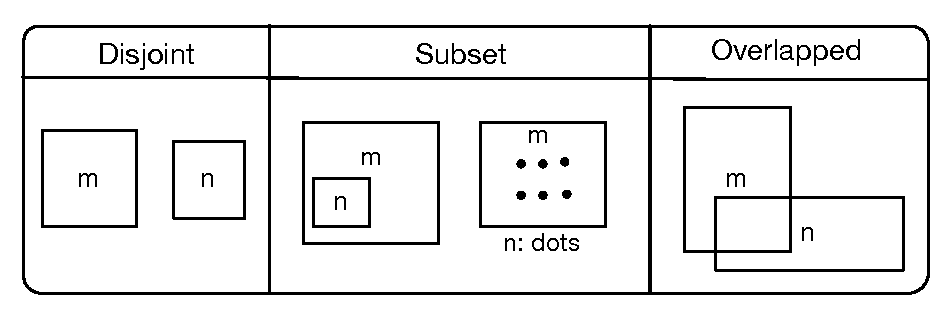
\includegraphics[scale=0.55]{figures/patterns.pdf}
\vspace{-0.1in}
\caption{Communication patterns}
\vspace{-0.1in}
\label{fig:patterns}
\end{figure}

\begin{itemize}
\item All to many, many to all
\item I/O Aggregation: a special case of All to many (or many to many)
\item Many to many: disjoint/exclusive
\item Many to many: subset
\item Many to many: partially joint (not subset, not disjoint)
\item Many to many: sparse
\end{itemize}

\subsection{All to many or Many to all}
